\chapter{Analytic Number Theory: Continuous Tools for Discrete Primes}

\section{A Counting Game That Gets Harder}

During break, four pupils play a counting game: the first says ``$2$'', and each following player names the next prime: $3$, $5$, $7$, $11$, $13$, and so on. At first they compete to answer; near fifty they start counting on their fingers; near a hundred someone reaches for scrap paper to try divisions. The game has a curious feel: initially primes are densely packed, appearing every one or two numbers, but farther along, the empty stretches widen and the waiting grows longer.

Another scene unfolds out of sight. Whenever you pay by phone, your browser and the bank's server exchange keys. One of the most popular public-key schemes begins by finding two large primes hundreds of digits long. How does a computer find them? Not by memorising a table: listing every prime of that size would require more than all the atoms in the universe. Its method is charmingly simple: choose a large number at random, test whether it is prime, and if not, try another until one works. This relies on a background fact: even hundreds of digits up the number line, primes are sparse but not vanishingly so. On average, a few hundred attempts find one.

Two questions emerge. We have already answered the first: do primes run out? No; Euclid proved their infinitude over two thousand years ago. The second is much subtler, and explains why our game grows harder:

\begin{quote}
Primes become sparser farther along. But how sparse? Is there a pattern to their thinning? Can a formula tell us roughly the density of primes near a number $x$?
\end{quote}

This sounds more like statistics or physics than a familiar integer problem. Integers jump one by one; they are discrete. Density, patterns, and formulas belong to the world of continuous variation. Analytic number theory does precisely this apparently unreasonable thing: it uses continuous tools---logarithms, integrals, infinite series, and even complex numbers---to study utterly discrete primes. Remarkably, this route not only works, but leads to mathematics' most famous unsolved mystery.

\section{A First Guess: Why a Fixed Share Does Not Work}

Begin with intuition. There are $25$ primes below a hundred, a quarter of the numbers. The natural guess is that primes occupy about a quarter of the integers farther along too, perhaps gradually a little less. In other words, prime density is approximately a fixed proportion.

Count a little farther and this guess collapses. Patiently extend the prime table, or consult one already made: up to $100$ there are $25$ primes, density $25\%$; up to $1000$ there are $168$, density $16.8\%$; up to $10000$ there are $1229$, only $12.3\%$. Density is not fluctuating around a fixed value, but steadily declining. The table rejects every fixed-proportion guess.

A second intuition asks whether density falls like $\dfrac{1}{x}$: near $x$, perhaps there is about $1$ prime in every $x$ numbers. This falls too quickly. It predicts only $1$ prime per $1000$ numbers near $1000$, yet there are actually $168$ primes up to $1000$, averaging $1$ in fewer than $6$ numbers. The real decline is much slower than $\dfrac{1}{x}$, but much faster than a fixed proportion. It lies somewhere in between.

\begin{fanli}
``Primes grow sparser, so far enough along there will be extremely long prime-free stretches, longer than any prescribed length. That means primes are effectively finite.''

The first part is true: we will soon prove that arbitrarily long runs of composite numbers exist. The second is false. Sparsity is not disappearance. Euclid's proof guarantees primes ahead however far you travel. Intuitively ``too sparse to see'' and logically ``none remain'' are different claims, a distinction we must watch carefully throughout this chapter.
\end{fanli}

A fixed proportion fails, and so does $\dfrac{1}{x}$. We need a new, slowly decaying function as a candidate density. You have already met it in Part III: the logarithm.

\section{Building a Prime Counter}

To discuss density, first choose a measuring tool. Our first new invention is a counting function:

\begin{dingyi}[Prime-counting function]
For any positive real number $x$, let $\pi(x)$ denote the number of primes no greater than $x$. For example, $\pi(10)=4$ (the primes are $2,3,5,7$), and $\pi(100)=25$.
\end{dingyi}

This $\pi$ is not the circle constant; it borrows the Greek letter corresponding to ``p'', for prime. The notation solves a problem: instead of vaguely saying that primes seem scarcer, we can say $\pi(100)=25$ and $\pi(1000)=168$, turning impressions into numbers that can be compared and plotted.

What does $\pi(x)$ look like? A staircase: it stays flat as $x$ passes composite numbers and jumps one step at every prime. Moving right, it only rises, never falls; because primes are infinite, the stairs continue forever without reaching a top.

\begin{center}
\begin{tikzpicture}[scale=1.0]
  \draw[->] (0,0) -- (6.5,0) node[below left] {$x$};
  \draw[->] (0,0) -- (0,4.2) node[below left] {$\pi(x)$};
  \draw[thick,blue!60!black]
    (0,0) -- (0.4,0) -- (0.4,0.35) -- (0.6,0.35) -- (0.6,0.7)
    -- (1.0,0.7) -- (1.0,1.05) -- (1.4,1.05) -- (1.4,1.4)
    -- (2.2,1.4) -- (2.2,1.75) -- (2.6,1.75) -- (2.6,2.1)
    -- (3.4,2.1) -- (3.4,2.45) -- (3.8,2.45) -- (3.8,2.8)
    -- (4.6,2.8) -- (4.6,3.15) -- (5.8,3.15) -- (5.8,3.5) -- (6.3,3.5);
  \foreach \p/\v in {0.4/2, 1.0/5, 2.2/11, 3.4/17, 4.6/23, 5.8/29}
    \node[below] at (\p,0) {\scriptsize $\v$};
  \node[right] at (6.3,3.5) {\scriptsize One step per prime};
\end{tikzpicture}
\end{center}

This counter is purely discrete: its uneven steps reveal no smooth pattern. Yet something magical happens from a distance: the jagged staircase follows a smooth curve. To describe that curve we need our second protagonist, the natural logarithm $\ln x$.

Recall where logarithms come from. The exponential relations $10^{2}=100$ and $10^{3}=1000$ tell us that $\lg 100=2$ and $\lg 1000=3$. Logarithms translate multiplication into addition and grow extremely slowly: multiplying $x$ by ten adds only one to $\lg x$. Mathematicians prefer the natural logarithm $\ln x$, with base $e\approx2.718$, because it is especially convenient in calculus. The area under $y=\dfrac{1}{t}$ from $1$ to $x$ is exactly $\ln x$. This identity as an area will soon prove useful.

Our third tool is a famous series:

\[
1+\frac12+\frac13+\frac14+\frac15+\cdots
\]

This is the harmonic series. Its terms shrink towards zero, yet their sum is infinite! A clever grouping reveals why. Put $\frac12$ alone; group $\frac13+\frac14$, whose two terms are each at least $\frac14$, giving at least $\frac12$; group the four terms from $\frac15$ to $\frac18$, each at least $\frac18$, again giving at least $\frac12$; then take eight terms, sixteen, and so on. Every group contributes at least $\frac12$. Infinitely many contributions of $\frac12$ clearly diverge to infinity. The lesson: tending to zero does not mean having a finite sum.

A crucial quantitative fact is that the first $n$ terms sum to approximately $\ln n$. This is unsurprising: $\ln n$ is the area under $y=\frac1t$, and $1+\frac12+\cdots+\frac1n$ adds rectangles of width $1$ and height $\frac1k$ covering that area. The rectangular sum cannot differ from the area by much. Roughly:

\[
1+\frac12+\frac13+\cdots+\frac1n \;\approx\; \ln n.
\]

Our three tools are on the table: the staircase counter $\pi(x)$, the slow logarithm $\ln x$, and the area bridge connecting logarithms with sums of reciprocals. It is time for the chapter's central story.

\section{The Prime Number Theorem: Order in Sparsity}

Late in the eighteenth century, the young Gauss received an intriguing gift: a logarithm table with a prime table in its appendix. He reportedly compared the two repeatedly and noticed something strange: the rhythm of prime density matched the rhythm of logarithmic growth. He guessed that near $x$, every $\ln x$ consecutive integers contain about $1$ prime. In other words, prime density near $x$ is approximately $\dfrac{1}{\ln x}$.

If density is $\dfrac{1}{\ln x}$, the total primes up to $x$ should result from accumulating this density from $2$ to $x$. In integral language, the smooth curve is $\displaystyle\int_2^x \frac{\mathrm{d}t}{\ln t}$. A rougher but easier approximation is $\dfrac{x}{\ln x}$. Gauss's guess was eventually proved correct, becoming the prime number theorem:

\begin{dingli}[Prime number theorem]
As $x$ grows larger,
\[
\pi(x)\;\approx\;\frac{x}{\ln x},
\]
meaning precisely that the ratio $\pi(x)\big/\dfrac{x}{\ln x}$ tends to $1$ as $x$ increases without bound.
\end{dingli}

\begin{zhu}
Gauss guessed this law in the late eighteenth century, but its proof took another hundred years. Only in $1896$ did Hadamard and de la Vallee Poussin independently prove it. Their weapons were not integer tricks but the theory of functions on the complex plane, the subject of this chapter's second half. The proof lies beyond this book, but we can test the theorem ourselves in a table.
\end{zhu}

Try it: $\ln 100\approx4.6$, $\ln 1000\approx6.9$, $\ln 10^{6}\approx13.8$, and $\ln 10^{9}\approx20.7$. Substitute into $\dfrac{x}{\ln x}$ and compare with the true $\pi(x)$:

\begin{center}
\begin{tabular}{crrc}
\toprule
$x$ & $\pi(x)$ & $x/\ln x$ (rounded) & Ratio $\pi(x)/(x/\ln x)$ \\
\midrule
$10^{2}$ & $25$ & $22$ & $1.15$ \\
$10^{3}$ & $168$ & $145$ & $1.16$ \\
$10^{4}$ & $1229$ & $1086$ & $1.13$ \\
$10^{5}$ & $9592$ & $8686$ & $1.10$ \\
$10^{6}$ & $78498$ & $72382$ & $1.08$ \\
$10^{9}$ & $50847534$ & $48254942$ & $1.05$ \\
\bottomrule
\end{tabular}
\end{center}

Look at the rightmost column: $1.15,1.16,1.13,1.10,1.08,1.05$, inching slowly towards $1$. This is what a ratio tending to $1$ looks like in practice: unhurried, but never stopping or turning back. A table is not a proof, as we will emphasise again, but it turns the claim that prime sparsity follows a precise law into visible numbers.

Back in our counting game, the prime number theorem says that the average gap near $x$ is roughly $\ln x$. Near $100$, a prime appears about every $4.6$ numbers; near $10^{6}$, about every $13.8$; at astronomical numbers hundreds of digits long, every few hundred. This explains why a computer finds a large prime after a few hundred random trials. Cryptographers are not merely lucky: the prime number theorem supports them.

\begin{shuyu}{Prime number theorem}
\textbf{Intuition:} Primes grow sparser, but $\ln x$ precisely controls the rhythm: density near $x$ is about $1/\ln x$.\\
\textbf{Formal statement:} $\pi(x)/(x/\ln x)\to 1$ as $x$ increases without bound.\\
\textbf{Example:} At $x=10^{6}$, $x/\ln x\approx72382$, while the true count is $\pi(x)=78498$. The difference is only about $8\%$, and the percentage shrinks as $x$ grows.
\end{shuyu}

Be careful: an average gap of roughly $\ln x$ is an average, not a rule for every stretch. Actual gaps fluctuate wildly. Some primes differ by only $2$, such as $29$ and $31$, or $41$ and $43$, called twin primes. Elsewhere hundreds or thousands of composites occur consecutively. In fact, the empty stretches can be arbitrarily long:

\begin{dingli}[Prime gaps can be arbitrarily large]
For every positive integer $n$, there exist $n$ consecutive positive integers none of which is prime.
\end{dingli}

\begin{proof}
Choose the large number $N=(n+1)!$, the product $1\times2\times3\times\cdots\times(n+1)$. Consider these $n$ numbers just beyond $N$:
\[
N+2,\ N+3,\ N+4,\ \dots,\ N+(n+1).
\]
For $N+2$, the number $N$ contains a factor $2$, since the factorial includes $2$, so $N+2$ is divisible by $2$ and composite. Similarly, $N+3$ is divisible by $3$ because $N$ contains a factor $3$. In general, for every $k$ from $2$ to $n+1$, the number $N$ contains $k$ as a factor. Thus $N+k$ is divisible by $k$ and clearly larger than $k$, hence composite. All $n$ consecutive integers from $N+2$ to $N+(n+1)$ are composite.
\end{proof}

This is a purely constructive proof: make the factorial large enough for the desired gap. For $1000$ consecutive composites, take $1001!$ plus $2$ through $1001!$ plus $1001$, a ``prime desert'' of astronomical length. Yet twin primes seemingly keep appearing forever: $3$ and $5$, $11$ and $13$, $\dots$, $101$ and $103$, $\dots$. Mathematicians conjecture infinitely many pairs: the famous twin prime conjecture remains neither proved nor disproved. In $2013$, Yitang Zhang proved infinitely many prime pairs differ by at most seventy million; worldwide collaboration subsequently reduced the bound to $246$. From $246$ to $2$ seems a short step, but nobody has crossed it.

The picture is therefore this: gaps grow on average, controlled by $\ln x$; individual gaps can be arbitrarily wide; and twins separated by $2$ seem never to disappear. Average regularity and individual unpredictability coexist. To know how orderly primes really are, $\pi(x)\approx x/\ln x$ is not enough. We must ask about the error: is the difference between $\pi(x)$ and $\dfrac{x}{\ln x}$ erratic, or governed by something deeper? This brings us to mathematics' most mysterious doorway.

\section{A Series Machine That Tunes In to Primes}

Turn from the table to a machine. In the eighteenth century, Euler studied the infinite series

\[
\zeta(s)\;=\;1+\frac{1}{2^{s}}+\frac{1}{3^{s}}+\frac{1}{4^{s}}+\cdots
\]

For now, take $s$ to be real and greater than $1$. At $s=1$, this is the divergent harmonic series; at $s=2$, it converges to $\dfrac{\pi^{2}}{6}$, itself a legendary result: the circle constant emerges from reciprocal squares of integers. Euler's key observation was that this seemingly unrelated series is entirely determined by primes. The reason is the fundamental theorem of arithmetic: every integer factors uniquely into primes. Factor each denominator, regroup the terms, and use geometric-series summation to turn addition into multiplication:

\[
1+\frac{1}{2^{s}}+\frac{1}{3^{s}}+\frac{1}{4^{s}}+\cdots
\;=\;
\frac{1}{1-2^{-s}}\times\frac{1}{1-3^{-s}}\times\frac{1}{1-5^{-s}}\times\frac{1}{1-7^{-s}}\times\cdots
\]

The right-hand side is an infinite product over every prime. This Euler product formula is the chapter's deepest line of poetry: all integers sing on the left, while each prime plays its own instrument on the right. The additive world of integers and the multiplicative world of primes are two expressions of the same machine.

A corollary follows immediately. Let $s$ tend to $1$: the left-hand series diverges to infinity. If primes were finite in number, the right-hand side would be a finite product of finite fractions, a contradiction. Thus primes must be infinite: Euler's product provides a proof with a completely different flavour. A finer calculation shows that the sum of all prime reciprocals,

\[
\frac12+\frac13+\frac15+\frac17+\frac1{11}+\cdots
\]

also diverges, as slowly as roughly $\ln(\ln x)$. Savour that result: primes have enough weight among the integers that even their reciprocal sum cannot be contained. Compared with squares, whose $\sum\frac{1}{n^2}$ converges, primes are much denser. Their infinitude is not a marginal affair; it has real substance.

\section{Riemann's Astonishing Leap: Sending $s$ into the Complex Plane}

Euler's machine requires $s>1$; otherwise the series will not converge. In $1859$, Riemann published just one short, eight-page paper, yet changed mathematical history by asking whether $\zeta(s)$ could be extended to the whole complex plane.

\begin{shuyu}{Riemann $\zeta$ function}
\textbf{Intuition:} A machine taking complex inputs, driven for $s>1$ by $1+2^{-s}+3^{-s}+\cdots$. Analytic continuation extends it to almost the entire complex plane.\\
\textbf{Part of the formal definition:} $\zeta(s)=\sum_{n=1}^{\infty} n^{-s}$ when the real part of $s$ exceeds $1$, then uniquely extended elsewhere, ``blowing up'' only at $s=1$.\\
\textbf{Example:} $\zeta(2)=\dfrac{\pi^{2}}{6}$; under continuation, $\zeta(-1)$ receives the value $-\dfrac{1}{12}$. This does not mean that $1+2+3+\cdots$ genuinely equals $-\frac{1}{12}$: it is the continued function's value there. These must not be confused.
\end{shuyu}

The difficulty is that the series converges only where the real part exceeds $1$; outside that region, $1+2^{-s}+3^{-s}+\cdots$ ceases to behave. Mathematicians use ingenious methods---roughly, rewriting the series indirectly into a convergent form, then proving that the resulting function is the unique appropriate extension---to give $\zeta$ a definite meaning everywhere except $s=1$. This technique, analytic continuation, belongs to complex analysis and lies beyond this book. Remember its valuable uniqueness: like extending a circular arc along its own curvature, there is just one natural continuation.

With the function in hand, Riemann asked which inputs produce zero: where are the solutions of $\zeta(s)=0$? Zeros are a function's ``genes'': just as roots determine a polynomial, zeros largely determine an analytic function. Calculation shows that the negative even integers $-2,-4,-6,\dots$ are zeros, called trivial zeros, with little surprise attached. The real secret lies in the vertical critical strip, where real parts lie between $0$ and $1$. It contains infinitely many nontrivial zeros, and Riemann calculated that the first few have real part exactly $\dfrac12$:

\[
\frac12+14.13\,\mathrm{i},\qquad
\frac12+21.02\,\mathrm{i},\qquad
\frac12+25.01\,\mathrm{i},\qquad\dots
\]

\begin{center}
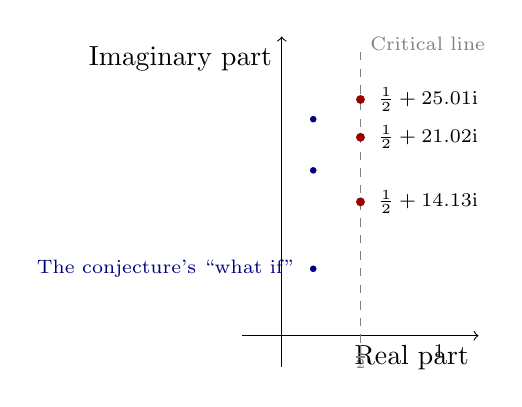
\begin{tikzpicture}[scale=1.0]
  \draw[->] (-0.5,0) -- (2.5,0) node[below left] {Real part};
  \draw[->] (0,-0.4) -- (0,3.8) node[below left] {Imaginary part};
  \draw[dashed,gray] (1,-0.3) -- (1,3.6);
  \node[below,gray] at (1,0) {\scriptsize $\frac12$};
  \node[below] at (2,0) {\scriptsize $1$};
  \node[above right,gray] at (1,3.5) {\scriptsize Critical line};
  \foreach \y in {1.7, 2.52, 3.0}
    \fill[red!60!black] (1,\y) circle (1.6pt);
  \node[right] at (1.1,1.7) {\scriptsize $\frac12+14.13\mathrm{i}$};
  \node[right] at (1.1,2.52) {\scriptsize $\frac12+21.02\mathrm{i}$};
  \node[right] at (1.1,3.0) {\scriptsize $\frac12+25.01\mathrm{i}$};
  \foreach \y in {0.85, 2.1, 2.75}
    \fill[blue!50!black] (0.4,\y) circle (1.2pt);
  \node[left,blue!50!black] at (0.3,0.85) {\scriptsize The conjecture's ``what if''};
\end{tikzpicture}
\end{center}

Why do zeros concern primes? Through Euler's product, $\zeta$ contains information about every prime, and its zeros are knobs for extracting that information. Riemann's eight-page paper gave a remarkable formula, whose proof was completed later: $\pi(x)$ can be expressed as a smooth main term plus a correction wave from each nontrivial zero. The larger a zero's real part, the larger its oscillation, and the harder it is to control the deviation of $\pi(x)$ from the smooth curve. The question of prime regularity becomes precisely the geometric question of where zeros lie.

Riemann turned his computed observations into a conjecture:

\begin{quote}
\textbf{Riemann hypothesis (1859, still unproved):} Every nontrivial zero of $\zeta$ has real part $\dfrac12$: they all lie neatly on one vertical line.
\end{quote}

Notice the wording: a \textbf{conjecture}, not a theorem. Over more than 160 years, computers have checked over ten trillion nontrivial zeros, all on this line. Countless mathematicians have sought a proof, accumulating mountains of equivalent statements and consequences, yet no proof has appeared. It is one of the Clay Mathematics Institute's seven Millennium Prize Problems, with a million-dollar reward.

Why does the hypothesis matter? It governs the prime number theorem's error. Mathematicians have proved that the deviation between $\pi(x)$ and the smooth curve is controlled entirely by the real parts of nontrivial zeros. If the hypothesis holds, this deviation is squeezed to its minimum, roughly bounded by the order of $\sqrt{x}\,\ln x$. Relative to $x$, this is like measuring the Earth--Moon distance with an error below a kilometre. Conversely, even one zero off the critical line would create much larger-than-expected irregular fluctuations in prime distribution. In everyday language: \textbf{primes are mischievous, but within limits; one straight line keeps their randomness in check.}

\begin{fanli}
``Computers have checked ten trillion zeros on the critical line, so the Riemann hypothesis is essentially settled; only a formality remains.''

This is the classic mistake of treating experiment as proof. There are infinitely many nontrivial zeros; however many we check, they are a cup of water from an infinite ocean. Mathematics offers harsh lessons: some statements hold for unimaginably large numbers, then first fail farther beyond human reach. Prime-distribution research has genuinely encountered reversals only at enormous scales. Experiments inspire conjectures, build confidence, and find counterexamples; only proof guarantees every case. This is the weight of ``analytic'' in the chapter title: the demand is for argument, not statistics.
\end{fanli}

\begin{lianjie}
Looking back, we have braided together several earlier threads: Chapter 9's limits, with a ratio tending to $1$; Chapter 11's series and integrals, including the harmonic series and the area meaning of $\ln x$; Chapter 12's complex numbers, used to continue $\zeta$; Chapter 13's fundamental theorem of arithmetic, underpinning Euler's product; and Chapter 14's computational experiments, including prime tables and sieves. Looking ahead, the Riemann hypothesis's claim that all zeros lie on one line already gestures towards Chapter 16's topology through shape and position. Public-key cryptography is prime distribution's most concrete practical application: it relies both on finding primes easily, with density guaranteed by the prime number theorem, and on factoring large numbers being difficult, with no fast algorithm yet known.
\end{lianjie}

\section{Count for Yourself: What Experiments Can and Cannot Do}

\begin{shiyan}
Prepare a grid of the numbers $1$ to $100$ and perform the sieve of Eratosthenes by hand: circle $2$ and cross out its multiples; circle the next survivor, $3$, and cross out its multiples; repeat for $5$ and $7$. Up to $100$, sieving only to $\sqrt{100}=10$ suffices---why? The survivors are all primes up to $100$. Count them: are there $25$?

Record consecutive prime gaps: $3-2=1$, $5-3=2$, $7-5=2$, $11-7=4$, and so on. Put them in a row and answer:
\begin{enumerate}
  \item What is the largest gap, and where does it occur?
  \item How many twin prime pairs have gap $2$?
  \item What is the approximate average gap? Is it close to $\ln 100\approx 4.6$?
\end{enumerate}
With a calculator or computer, extend the experiment to $1000$ and observe the average moving towards $\ln 1000\approx 6.9$. If you can, write a short programme of a dozen or so lines: two nested loops imitate circling and crossing out, letting the computer count to a hundred thousand.
\end{shiyan}

Afterwards, pause: what exactly have the table and programme proved? They tell you that up to $100$, the average prime gap is about $4.3$, the same order as $\ln 100$. This is an observation, a sample of the prime number theorem at $x=100$. It does not, and cannot, prove that a ratio tends to $1$. The same logic applies to the Riemann hypothesis: ten trillion checks remain an experiment. Mathematics has three levels, all represented here: \textbf{experiment}, including sieves, tables, and zero calculations, supplies clues; \textbf{conjecture}, including twin primes and the Riemann hypothesis, points the way; \textbf{proof}, including Euclid, the factorial construction, and the prime number theorem, provides guarantees. Confusing these levels is among number theory's easiest traps and most important lessons.

\begin{toolbox}
New tools from this chapter:
\begin{itemize}
  \item \textbf{Counting function $\pi(x)$}: Turn the impression of thinning primes into a function to plot and compare.
  \item \textbf{Natural logarithm $\ln x$}: One of the slowest-growing elementary functions, the scale of prime density and also the area under $y=\frac1t$.
  \item \textbf{Harmonic series and divergence}: Terms tending to zero do not guarantee convergence; the first $n$ terms sum to roughly $\ln n$.
  \item \textbf{Euler product}: $\sum n^{-s}=\prod_{p}(1-p^{-s})^{-1}$ translates between integer addition and prime multiplication.
  \item \textbf{$\zeta$ and analytic continuation}: Extend the series machine to the complex plane; zero locations control prime-distribution error.
  \item \textbf{Distinguishing experiment, conjecture, and proof}: Tables inspire conjectures, conjectures guide proofs, and only proofs guarantee results.
\end{itemize}
\end{toolbox}

\begin{pandeng}
For further exploration, remember these signposts: \textbf{Chebyshev functions} and elementary proofs of the prime number theorem, given independently by Selberg and Erdos in $1949$ without complex analysis; the \textbf{logarithmic integral} $\mathrm{Li}(x)$, closer to $\pi(x)$ than $x/\ln x$; \textbf{analytic continuation} and complex analysis, the true language of Riemann's paper; modern \textbf{sieve methods}, supporting prime-gap research after Yitang Zhang; and \textbf{zero computations}, pinning ten trillion zeros to the critical line one by one with fast computers. Any of these could keep you in libraries or online for a whole summer.
\end{pandeng}

\section*{Questions to Think About}

\textbf{Observation}
\begin{sikao}
  \item Record prime gaps up to $100$ again and identify every record gap, larger than all preceding gaps. Look at the primes at those positions and guess where the next record might occur. \emph{Hint: a record gap marks a relatively long composite desert. Think about the factorial construction: are deserts likelier near specially structured numbers or just anywhere?}
  \item Inspect the table's ratio column from $10^{2}$ to $10^{9}$. How much must $x$ multiply for each small decrease in the ratio? Get a feel for how slowly it tends to $1$. \emph{Hint: multiplying $x$ by $10$ moves the ratio by only a fraction of a percentage point. It is not lack of effort; $\ln x$ grows very reservedly.}
\end{sikao}

\textbf{Proof}
\begin{sikao}
  \item Prove that $1000$ consecutive positive integers can all be composite. Explain roughly how high your constructed interval lies. \emph{Hint: choose an appropriate factorial for $N=(n+1)!$ and check why every $N+k$ is composite.}
  \item Without consulting a table, prove that a sufficiently long consecutive block of harmonic-series terms, however far out it begins, can have sum greater than $10$. \emph{Hint: recall the grouping argument, where each group contributes at least $\frac12$. About how many groups exceed $10$?}
\end{sikao}

\textbf{Challenge}
\begin{sikao}
  \item Euler's product showed that finitely many primes would give a contradiction as $s\to1$. Go further: explain why divergence of prime reciprocals seems almost inevitable from the product formula. \emph{Hint: take logarithms to turn the product into a sum. As $s\to1$, the left side blows up; expanding the terms $\ln(1-p^{-s})$ on the right gives leading terms $\frac1p$. This requires fluency in turning products into sums with logarithms, so getting stuck is normal.}
\end{sikao}

\section*{The Door to the Next Chapter}

We crossed a boundary: continuous, smooth analysis interrogated discrete, individual primes. Look again at the zero diagram. One detail deserves another glance: the Riemann hypothesis says that infinitely many mysterious points all lie on \textbf{the same straight line}.

``Lying on a line'', ``forming a loop'', ``having a hole'': we have used these phrases casually several times. But what is a line? What is a hole? Replace the complex plane by a rubber sheet and allow stretching, bending, and twisting without tearing or joining broken pieces: is the critical line still a line? Under rules permitting deformation but no tearing, why are a coffee cup and a doughnut the same kind of object, yet different from a sphere?

Number theory advances through counting and proof. These questions need a subject devoted to properties that survive deformation. It ignores lengths and angles, asking only about connections, passages, and holes. This is the world of the next chapter: topology.
